%% Exemplo de utilizacao do estilo de formatacao normas-utf-tex (http://normas-utf-tex.sourceforge.net)
%% Autores: (200?-2011) Hugo Vieira Neto (hvieir@utfpr.edu.br)
%%          (200?-2011) Diogo Rosa Kuiaski (diogo.kuiaski@gmail.com)
%%          (2011-2012) Marcos Talau <talau@users.sourceforge.net>
%% Colaborador:
%%          (2011) César M. Vargas Benitez <cesarvargasb@gmail.com>
%%          (2015) Glauber Gomes de Oliveira Brante <gbrante@utfpr.edu.br>

\documentclass[openright]{normas-utf-tex} %openright = o capitulo comeca sempre em paginas impares
%\documentclass[oneside]{normas-utf-tex} %oneside = para documentos com numero de paginas menor que 100 (apenas frente da folha)

% force A4 paper format
\special{papersize=210mm,297mm}
\usepackage[hidelinks,plainpages=true, bookmarks=true, breaklinks, pdfstartview=FitH,pdftitle={Nome da Teste},pdfauthor={Nome do autor},pdfsubject={Assunto do documento},pdfkeywords={Palavras-chave}]{hyperref}
\usepackage[hyphenbreaks]{breakurl}
\urlstyle{same}
%configuracao correta das referencias bibliograficas.
\usepackage[alf,abnt-emphasize=bf,bibjustif,recuo=0cm,abnt-etal-cite=2,abnt-etal-list=0,abnt-thesis-year=both]{abntcite}

\usepackage[brazil]{babel} % pacote portugues brasileiro
\usepackage[latin1]{inputenc} % pacote para acentuacao direta
\usepackage{amsmath,amsfonts,amssymb} % pacote matematico
\usepackage{graphicx} % pacote grafico
%\usepackage{times} % fonte times (substituida pelos dois comandos abaixo - padrao LATEX)
\usepackage[T1]{fontenc}
\usepackage{lmodern}
\usepackage[final]{pdfpages} % adicao da ata
\usepackage[
    type={CC},
    modifier={by-nc-sa},
    version={4.0},
    imageposition={right},
]{doclicense}

% ---------- Preambulo ----------
\instituicao{Universidade Tecnológica Federal do Paraná} % nome da instituicao
\programa{Programa de Pós-Graduação em Sistemas de Energia} % nome do programa
\area{Automação e Sistemas de Energia} % area de concentracao

\documento{Dissertação} % [Dissertacao] ou [Tese]
\documentoingles{Thesis}
\nivel{Mestrado} % [Mestrado] ou [Doutorado]
\curso{Sistemas de Energia}
\titulacao{Mestre} % [Mestre] ou [Doutor]

\titulo{Sistema de localização em ambientes internos por meio de bluetooth 5.1 utilizando RSSI e AoA.} % titulo do trabalho em portugues
\title{Indoor positioning system using RSSI and AoA from Bluetooth 5.1 Direction Finding.} % titulo do trabalho em ingles

\autor{Andrey Fabris} % autor do trabalho
\cita{FABRIS, Andrey} % sobrenome (maiusculas), nome do autor do trabalho

\palavraschave{Localização interna. Bluetooth. .Filtro de Kalman. Ângulo de Chegada.} % palavras-chave do trabalho
\keywords{Indoor Positioning. Bluetooth. Kalman Filter. Angle of Arrival} % palavras-chave do trabalho em ingles

\comentario{\UTFPRdocumentodata\ apresentada ao \UTFPRprogramadata\ da \ABNTinstituicaodata\ como requisito parcial para obtenção do título de ``\UTFPRtitulacaodata\ em Engenharia Elétrica'' -- Área de Concentração: \UTFPRareadata.}

\orientador{Ohara Kerusauskas Rayel} % nome do orientador do trabalho
%\orientador[Orientadora:]{Nome da Orientadora} % <- no caso de orientadora, usar esta sintaxe
\coorientador{João Luiz Rebelatto} % nome do coorientador do trabalho, caso exista
%\coorientador[Coorientadora:]{Nome da Coorientadora} % <- no caso de co-orientadora, usar esta sintaxe

\local{Curitiba} % cidade
\data{2024} % ano


% desativa hifenizacao mantendo o texto justificado.
\tolerance=1
\emergencystretch=\maxdimen
\hyphenpenalty=10000
\hbadness=10000
\sloppy


%---------- Inicio do Documento ----------
\begin{document}
\pdfstringdefDisableCommands{%
	\let\MakeUppercase\relax
}
\capa % geracao automatica da capa
\folhaderosto % geracao automatica da folha de rosto


% insercao da ATA
%\includepdf{ata.pdf}


% dedicatoria
\begin{dedicatoria}
Dedico esse trabalho à minha família, que sempre me apoiou e incentivou aos estudos.
\end{dedicatoria}

% agradecimentos (opcional)
\begin{agradecimentos}
Diversas pessoas contribuíram para tornar possível o desenvolvimento desta dissetação, dentre as quais ficam meus agradecimentos:

Ao professor orientador, Dr. Ohara Keusauskas Rayel, e coorientador, Dr. João Luiz Rebelatto, que desde o início acompanharam e deram toda a ajuda necessária para a elaboração deste trabalho.

Aos professores do PPGSE e demais departamentos de Pós-Graduações de UTFPR, que através de seus ensinamentos permitiu que obtivesse todos os conhecimentos para estar concluindo este trabalho e o mestrado.

À Universidade Tecnológica Federal do Paraná, por possibilitar o ingresso ao programa de pós-graduação e dispor de toda a estrutura para seus alunos  alcançarem todo o conhecimento desejado.

Aos familiares, por todo o apoio durante os momentos de estudos e motivação para que alcançássemos nossos sonhos.

Aos amigos, pelos momentos de lazer e trocas de informação e materiais em demonstrações de amizades.

E a todas as pessoas que fizeram parte direta ou indiretamente em minha formação, meu muito obrigado.
\end{agradecimentos}

% epigrafe (opcional)
\begin{epigrafe}
"Strive for perfection in everything you do. Take the best that exists and make it better. When it does not exist, design it." - Sir Henry Royce
\end{epigrafe}

%resumo
\begin{resumo}
Dentre as diversas técnicas de radiofrequência utilizadas para obtenção de localização, como Received Signal Strength Indication (RSSI), Time of Flight (ToF) e Angle of Arrival (AoA), que são combinadas com algoritmos para determinar o posicionamento de um alvo em ambientes internos , o AoA vem ganhando interesse desde sua incorporação ao Bluetooth Low Energy (BLE) 5.1, devido à sua precisão, baixo consumo de energia, baixo custo e facilidade de implementação. Este trabalho tem como objetivo reduzir o erro de posição estimada de um alvo através da multilateração baseada em RSSI, bem como a posição estimada usando AoA e RSSI empregando filtros estocásticos, e propor um sistema com maior precisão usando a saída filtrada combinada de ambas as técnicas. Assim, será possível ter um sistema de posicionamento interno (IPS) BLE 5.1 ??mais preciso e eficiente em comparação com outras técnicas utilizadas, que pode ser utilizado para localizar pessoas e bens em ambientes internos com baixo erro de estimativa. Para atingir esse objetivo, este trabalho utilizará um banco de dados de medições reais de RSSI e AoA de um nó alvo BLE 5.1 ??e um conjunto de antenas em um ambiente de 13,8x8m, fornecido pela comunidade acadêmica, e aplicará o Filtro de Kalman ao algoritmo de localização para reduzir o erro de estimativa. Os erros serão calculados utilizando o Root Mean Square Error (RMSE), e os resultados serão comparados com os da literatura. Espera-se alcançar alta precisão na estimativa da localização de um alvo usando RSSI e AoA e o sistema combinado proposto alcançará um erro de localização menor do que sistemas separados. A técnica de localização indoor apresentada neste trabalho pode ser utilizada para substituir IPS de alto custo ou baixa precisão em diversas aplicações nas indústrias, saúde, comércio, logística, entre outras áreas..
\end{resumo}

%abstract
\begin{abstract}
Among the various radiofrequency techniques used for obtaining location, such as Received Signal Strength Indication (RSSI), Time of Flight (ToF), and Angle of Arrival (AoA), which are combined with algorithms to determine the positioning of a target in indoor environments, AoA has been gaining interest since its incorporation into Bluetooth Low Energy (BLE) 5.1, due to its precision, low energy consumption, low cost, and ease of implementation. This work aims to reduce the estimated position error of a target through multilateration based on RSSI, as well as the estimated position using AoA and RSSI employing stochastic filters, and to propose a system with improved accuracy by using the combined filtered output of both techniques. Thus, it will be possible to have a more precise and efficient BLE 5.1 indoor positioning system (IPS) compared to other techniques used, which can be used to locate people and assets in indoor environments with low estimation error. To achieve this goal, this work will use a database of real RSSI and AoA measurements from a BLE 5.1 target node and a set of antennas in a 13.8x8m environment, provided by the academic community, and apply the Kalman Filter to the localization algorithm to reduce estimation error. Errors will be calculated using the Root Mean Square Error (RMSE), and the results will be compared with those in the literature. It is expected to achieve high accuracy in estimating the location of a target using RSSI and AoA and the proposed combined system will achieve a lower location error than separate systems. The indoor localization technique presented in this work can be used to replace high-cost or low-precision IPS in several applications in industries, healthcare, commerce, logistics, and other areas.
\end{abstract}

% listas (opcionais, mas recomenda-se a partir de 5 elementos)
\listadefiguras % geracao automatica da lista de figuras
\listadetabelas % geracao automatica da lista de tabelas
%\listadequadros % adivinhe :)
\listadesiglas % geracao automatica da lista de siglas
\listadesimbolos % geracao automatica da lista de simbolos

% sumario
\sumario % geracao automatica do sumario

% Pacotes necessários quando não se usa sumário
%\renewcommand{\chaptertitlepagestyle}{plainheader}
%\pagenumbering{arabic}



%---------- Inicio do Texto ----------
% recomenda-se a escrita de cada capitulo em um arquivo texto separado (exemplo: intro.tex, fund.tex, exper.tex, concl.tex, etc.) e a posterior inclusao dos mesmos no mestre do documento utilizando o comando \input{}, da seguinte forma:
%\input{intro.tex}
%\input{fund.tex}
%\input{exper.tex}
%\input{concl.tex}


\setcounter{page}{11}

%---------- Primeiro Capitulo ----------
\chapter{Introdução}
\label{chap:introducao}

O presente documento é um exemplo de uso do estilo de formatação \LaTeX\ elaborado para atender às Normas para Elaboração de Trabalhos Acadêmicos da UTFPR. O estilo de formatação {\ttfamily normas-utf-tex.cls} tem por base o pacote \textsc{abn}\TeX~-- cuja leitura da documentação \cite{abnTeX2009} é fortemente sugerida~-- e o estilo de formatação \LaTeX\ da UFPR.

Para melhor entendimento do uso do estilo de formatação {\ttfamily normas-utf-tex.cls}, aconselha-se que o potencial usuário analise os comandos existentes no arquivo \TeX\ ({\ttfamily modelo\_*.tex}) e os resultados obtidos no arquivo PDF ({\ttfamily modelo\_*.pdf}) depois do processamento pelo software \LaTeX\ + \textsc{Bib}\TeX~\cite{LaTeX2009,BibTeX2009}. Recomenda-se a consulta ao material de referência do software para a sua correta utilização~\cite{Lamport1986,Buerger1989,Kopka2003,Mittelbach2004}.

\section{Motivação}
\label{sec:motivacao}

Uma das principais vantagens do uso do estilo de formatação {\ttfamily normas-utf-tex.cls} para \LaTeX\ é a formatação \textit{automática} dos elementos que compõem um documento acadêmico, tais como capa, folha de rosto, dedicatória, agradecimentos, epígrafe, resumo, abstract, listas de figuras, tabelas, siglas e símbolos, sumário, capítulos, referências, etc. Outras grandes vantagens do uso do \LaTeX\ para formatação de documentos acadêmicos dizem respeito à facilidade de gerenciamento de referências cruzadas e bibliográficas, além da formatação~-- inclusive de equações  matemáticas~-- correta e esteticamente perfeita.

\section{Objetivos}
\label{sec:objetivos}

\subsection{Objetivo Geral}
\label{subsec:objetivoGeral}

Prover um modelo de formatação \LaTeX\ que atenda às Normas para Elaboração de Trabalhos Acadêmicos da UTFPR~\cite{UTFPR2008}.

\subsection{Objetivos Específicos}
\label{subsec:objetivosEspecificos}

\begin{itemize}
	\item Obter documentos acadêmicos automaticamente formatados com correção e perfeição estética.
	\item Desonerar autores da tediosa tarefa de formatar documentos acadêmicos, permitindo sua concentração no conteúdo do mesmo.
	\item Desonerar orientadores e examinadores da tediosa tarefa de conferir a formatação de documentos acadêmicos, permitindo sua concentração no conteúdo do mesmo.
\end{itemize}



%---------- Segundo Capitulo ----------
\chapter{Desenvolvimento}
\label{chap:desenv}

A seguir ilustra-se a forma de incluir figuras, tabelas, equações, siglas e símbolos no documento, obtendo indexação automática em suas respectivas listas. A numeração sequencial de figuras, tabelas e equações ocorre de modo automático. Referências cruzadas são obtidas através dos comandos {\ttfamily \textbackslash label\{\}} e {\ttfamily \textbackslash ref\{\}}. Por exemplo, não é necessário saber que o número deste capítulo é~\ref{chap:desenv} para colocar o seu número no texto. Isto facilita muito a inserção, remoção ou relocação de elementos numerados no texto (fato corriqueiro na escrita e correção de um documento acadêmico) sem a necessidade de renumerá-los todos.

\section{Figuras}
\label{sec:figuras}

Na figura~\ref{fig:dummy} é apresentado um exemplo de gráfico flutuante. Esta figura aparece automaticamente na lista de figuras. Para uso avançado de gráficos no \LaTeX, recomenda-se a consulta de literatura especializada~\cite{Goossens2007}.

\begin{figure}[!htb]
	\centering
	\caption[Exemplo de uma figura]{Exemplo de uma figura onde aparece uma imagem sem nenhum significado especial.}
	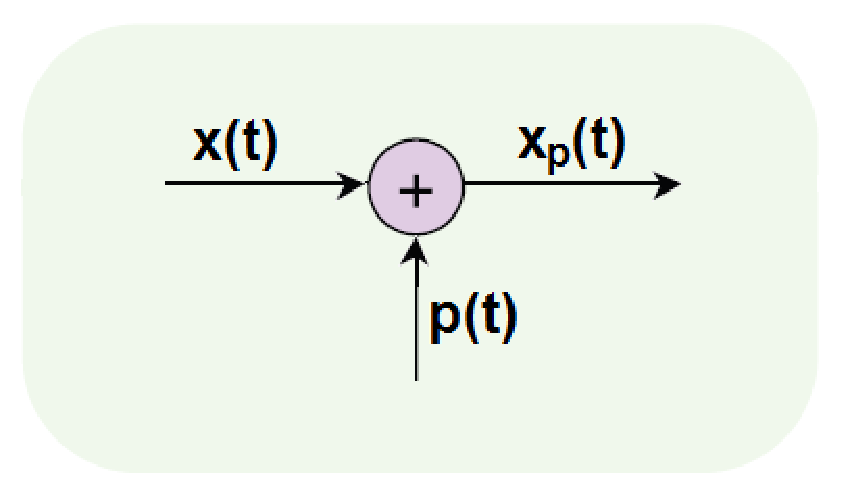
\includegraphics[width=5cm]{./dummy.eps} % <- formatos PNG, EPS e PDF	
	\fonte{Adaptado de \cite{abnTeX2009}}
	\label{fig:dummy}
\end{figure}


\section{Tabelas}
\label{sec:tabelas}

Também é apresentado o exemplo da tabela~\ref{tab:correlacao}, que aparece automaticamente na lista de tabelas. Informações sobre a construção de tabelas no \LaTeX\ podem ser encontradas na literatura especializada~\cite{Lamport1986,Buerger1989,Kopka2003,Mittelbach2004}.

\begin{table}[!htb]
	\centering
	\caption[Exemplo de uma tabela]{Exemplo de uma tabela mostrando a correlação entre x e y.}
	\label{tab:correlacao}
	\begin{tabular}{cc}
		\hline
		x & y \\
		\hline
		1 & 2 \\
		3 & 4 \\
		5 & 6 \\
		7 & 8 \\
		\hline
	\end{tabular}
	\fonte{Autoria própria.}
\end{table}



\section{Equações}
\label{sec:equacoes}

A transformada de Laplace é dada na equação~\eqref{eq:laplace}, enquanto a equação~\eqref{eq:dft} apresenta a formulação da transformada discreta de Fourier bidimensional\footnote{Deve-se reparar na formatação esteticamente perfeita destas equações!}.

\begin{equation}
X(s) = \int\limits_{t = -\infty}^{\infty} x(t) \, \text{e}^{-st} \, dt
\label{eq:laplace}
\end{equation}

\begin{equation}
F(u, v) = \sum_{m = 0}^{M - 1} \sum_{n = 0}^{N - 1} f(m, n) \exp \left[ -j 2 \pi \left( \frac{u m}{M} + \frac{v n}{N} \right) \right]
\label{eq:dft}
\end{equation}

\section{Siglas e símbolos}
\label{sec:siglasSimbolos}

O pacote \textsc{abn}\TeX\ permite ainda a definição de siglas e símbolos com indexação automática através dos comandos {\ttfamily \textbackslash sigla\{\}\{\}} e {\ttfamily \textbackslash simbolo\{\}\{\}}. Por exemplo, o significado das siglas \sigla{PPGSE}{Programa de Pós-Graduação em Sistemas de Energia}, \sigla{DAELT}{Departamento Acadêmico de Eletrotécnica} e \sigla{UTFPR}{Universidade Tecnológica Federal do Paraná} aparecem automaticamente na lista de siglas, bem como o significado dos símbolos \simbolo{$\lambda$}{comprimento de onda}, \simbolo{$v$}{velocidade} e \simbolo{$f$}{frequência} aparecem automaticamente na lista de símbolos. Mais detalhes sobre o uso destes e outros comandos do \textsc{abn}\TeX\ são encontrados na sua documentação específica~\cite{abnTeX2009}.


%---------- Terceiro Capitulo ----------
\chapter{Conclusão}
\label{chap:conclusao}

Espera-se que o uso do estilo de formatação \LaTeX\ adequado às Normas para Elaboração de Trabalhos Acadêmicos da UTFPR ({\ttfamily normas-utf-tex.cls}) facilite a escrita de documentos no âmbito desta instituição e aumente a produtividade de seus autores. Para usuários iniciantes em \LaTeX, além da bibliografia especializada já citada, existe ainda uma série de recursos~\cite{CTAN2009} e fontes de informação~\cite{TeX-Br2009,Wikibooks2009} disponíveis na Internet.

Recomenda-se o editor de textos Kile como ferramenta de composição de documentos em \LaTeX\ para usuários Linux. Para usuários Windows recomenda-se o editor \TeX nicCenter~\cite{TeXnicCenter2009} ou TexMaker. O \LaTeX\ normalmente já faz parte da maioria das distribuições Linux, mas no sistema operacional Windows é necessário instalar o software \textsc{MiK}\TeX~\cite{MiKTeX2009}.

Além disso, recomenda-se o uso de um gerenciador de referências como o JabRef~\cite{JabRef2009} ou Mendeley~\cite{Mendeley2009} para a catalogação bibliográfica em um arquivo \textsc{Bib}\TeX, de forma a facilitar citações através do comando {\ttfamily \textbackslash cite\{\}} e outros comandos correlatos do pacote \textsc{abn}\TeX. A lista de referências deste documento foi gerada automaticamente pelo software \LaTeX\ + \textsc{Bib}\TeX\ a partir do arquivo {\ttfamily reflatex.bib}, que por sua vez foi composto com o gerenciador de referências JabRef.

O estilo de formatação \LaTeX\ da UTFPR e este exemplo de utilização foram elaborados por Diogo Rosa Kuiaski (diogo.kuiaski@gmail.com) e Hugo Vieira Neto (hvieir@utfpr.edu.br), com contribuições de César Vargas Benitez. A adaptação para o PPGSE foi feita por Glauber Brante (gbrante@utfpr.edu.br). Sugestões de melhorias são bem-vindas.



%---------- Referencias ----------
\clearpage % this is need for add +1 to pageref of bibstart used in 'ficha catalografica'.
\label{bibstart}
\bibliography{reflatex} % geracao automatica das referencias a partir do arquivo reflatex.bib
\label{bibend}


%---------- Apendices (opcionais) ----------
\apendice
\chapter{Nome do Apêndice}
\label{chap:apendice}

Use o comando {\ttfamily \textbackslash apendice} e depois comandos {\ttfamily \textbackslash chapter\{\}}
para gerar títulos de apêndices.


% ---------- Anexos (opcionais) ----------
\anexo
\chapter{Nome do Anexo}
\label{chap:anexo}

Use o comando {\ttfamily \textbackslash anexo} e depois comandos {\ttfamily \textbackslash chapter\{\}}
para gerar títulos de anexos.


% --------- Ordenacao Afabetica da Lista de siglas --------
%\textbf{* Observa\c{c}\~oes:} a ordenacao alfabetica da lista de siglas ainda nao eh realizada de forma automatica, porem
% eh possivel se de realizar isto manualmente. Duas formas:
%
% ** Primeira forma)
%    A ordenacao eh feita com o auxilio do comando 'sort', disponivel em qualquer
% sistema Linux e UNIX, e tambem em sistemas Windows se instalado o coreutils (http://gnuwin32.sourceforge.net/packages/coreutils.htm)
% comandos para compilar e ordenar, supondo que seu arquivo se chame 'dissertacao.tex':
%
%      $ latex dissertacao
%      $ bibtex dissertacao && latex dissertacao
%      $ latex dissertacao
%      $ sort dissertacao.lsg > dissertacao.lsg.tmp
%      $ mv dissertacao.lsg.tmp dissertacao.lsg
%      $ latex dissertacao
%      $ dvipdf dissertacao.dvi
%
%
% ** Segunda forma)
%\textbf{Sugest\~ao:} crie outro arquivo .tex para siglas e utilize o comando \sigla{sigla}{descri\c{c}\~ao}.
%Para incluir este arquivo no final do arquivo, utilize o comando \input{arquivo.tex}.
%Assim, Todas as siglas serao geradas na ultima pagina. Entao, devera excluir a ultima pagina da versao final do arquivo
% PDF do seu documento.


%-------- Citacoes ---------
% - Utilize o comando \citeonline{...} para citacoes com o seguinte formato: Autor et al. (2011).
% Este tipo de formato eh utilizado no comeco do paragrafo. P.ex.: \citeonline{autor2011}

% - Utilize o comando \cite{...} para citacoeses no meio ou final do paragrafo. P.ex.: \cite{autor2011}



%-------- Titulos com nomes cientificos (titulo, capitulos e secoes) ----------
% Regra para escrita de nomes cientificos:
% Os nomes devem ser escritos em italico,
%a primeira letra do primeiro nome deve ser em maiusculo e o restante em minusculo (inclusive a primeira letra do segundo nome).
% VEJA os exemplos abaixo.
%
% 1) voce nao quer que a secao fique com uppercase (caixa alta) automaticamente:
%\section[nouppercase]{\MakeUppercase{Estudo dos efeitos da radiacao ultravioleta C e TFD em celulas de} {\textit{Saccharomyces boulardii}}
%
% 2) por padrao os cases (maiusculas/minuscula) sao ajustados automaticamente, voce nao precisa usar makeuppercase e afins.
% \section{Introducao} % a introducao sera posta no texto como INTRODUCAO, automaticamente, como a norma indica.


\end{document}
